% Options for packages loaded elsewhere
\PassOptionsToPackage{unicode}{hyperref}
\PassOptionsToPackage{hyphens}{url}
%
\documentclass[
  man]{apa6}
\usepackage{amsmath,amssymb}
\usepackage{lmodern}
\usepackage{iftex}
\ifPDFTeX
  \usepackage[T1]{fontenc}
  \usepackage[utf8]{inputenc}
  \usepackage{textcomp} % provide euro and other symbols
\else % if luatex or xetex
  \usepackage{unicode-math}
  \defaultfontfeatures{Scale=MatchLowercase}
  \defaultfontfeatures[\rmfamily]{Ligatures=TeX,Scale=1}
\fi
% Use upquote if available, for straight quotes in verbatim environments
\IfFileExists{upquote.sty}{\usepackage{upquote}}{}
\IfFileExists{microtype.sty}{% use microtype if available
  \usepackage[]{microtype}
  \UseMicrotypeSet[protrusion]{basicmath} % disable protrusion for tt fonts
}{}
\makeatletter
\@ifundefined{KOMAClassName}{% if non-KOMA class
  \IfFileExists{parskip.sty}{%
    \usepackage{parskip}
  }{% else
    \setlength{\parindent}{0pt}
    \setlength{\parskip}{6pt plus 2pt minus 1pt}}
}{% if KOMA class
  \KOMAoptions{parskip=half}}
\makeatother
\usepackage{xcolor}
\IfFileExists{xurl.sty}{\usepackage{xurl}}{} % add URL line breaks if available
\IfFileExists{bookmark.sty}{\usepackage{bookmark}}{\usepackage{hyperref}}
\hypersetup{
  pdftitle={Demanding resources: Similarity of perceptions for challenge and resource characteristics},
  pdfauthor={John Kulas1, Alicia Stachowski2, \& Renata Garcia Prieto Palacios Roji3},
  pdflang={en-EN},
  pdfkeywords={keywords},
  hidelinks,
  pdfcreator={LaTeX via pandoc}}
\urlstyle{same} % disable monospaced font for URLs
\usepackage{graphicx}
\makeatletter
\def\maxwidth{\ifdim\Gin@nat@width>\linewidth\linewidth\else\Gin@nat@width\fi}
\def\maxheight{\ifdim\Gin@nat@height>\textheight\textheight\else\Gin@nat@height\fi}
\makeatother
% Scale images if necessary, so that they will not overflow the page
% margins by default, and it is still possible to overwrite the defaults
% using explicit options in \includegraphics[width, height, ...]{}
\setkeys{Gin}{width=\maxwidth,height=\maxheight,keepaspectratio}
% Set default figure placement to htbp
\makeatletter
\def\fps@figure{htbp}
\makeatother
\setlength{\emergencystretch}{3em} % prevent overfull lines
\providecommand{\tightlist}{%
  \setlength{\itemsep}{0pt}\setlength{\parskip}{0pt}}
\setcounter{secnumdepth}{-\maxdimen} % remove section numbering
% Make \paragraph and \subparagraph free-standing
\ifx\paragraph\undefined\else
  \let\oldparagraph\paragraph
  \renewcommand{\paragraph}[1]{\oldparagraph{#1}\mbox{}}
\fi
\ifx\subparagraph\undefined\else
  \let\oldsubparagraph\subparagraph
  \renewcommand{\subparagraph}[1]{\oldsubparagraph{#1}\mbox{}}
\fi
\newlength{\cslhangindent}
\setlength{\cslhangindent}{1.5em}
\newlength{\csllabelwidth}
\setlength{\csllabelwidth}{3em}
\newlength{\cslentryspacingunit} % times entry-spacing
\setlength{\cslentryspacingunit}{\parskip}
\newenvironment{CSLReferences}[2] % #1 hanging-ident, #2 entry spacing
 {% don't indent paragraphs
  \setlength{\parindent}{0pt}
  % turn on hanging indent if param 1 is 1
  \ifodd #1
  \let\oldpar\par
  \def\par{\hangindent=\cslhangindent\oldpar}
  \fi
  % set entry spacing
  \setlength{\parskip}{#2\cslentryspacingunit}
 }%
 {}
\usepackage{calc}
\newcommand{\CSLBlock}[1]{#1\hfill\break}
\newcommand{\CSLLeftMargin}[1]{\parbox[t]{\csllabelwidth}{#1}}
\newcommand{\CSLRightInline}[1]{\parbox[t]{\linewidth - \csllabelwidth}{#1}\break}
\newcommand{\CSLIndent}[1]{\hspace{\cslhangindent}#1}
\ifLuaTeX
\usepackage[bidi=basic]{babel}
\else
\usepackage[bidi=default]{babel}
\fi
\babelprovide[main,import]{english}
% get rid of language-specific shorthands (see #6817):
\let\LanguageShortHands\languageshorthands
\def\languageshorthands#1{}
% Manuscript styling
\usepackage{upgreek}
\captionsetup{font=singlespacing,justification=justified}

% Table formatting
\usepackage{longtable}
\usepackage{lscape}
% \usepackage[counterclockwise]{rotating}   % Landscape page setup for large tables
\usepackage{multirow}		% Table styling
\usepackage{tabularx}		% Control Column width
\usepackage[flushleft]{threeparttable}	% Allows for three part tables with a specified notes section
\usepackage{threeparttablex}            % Lets threeparttable work with longtable

% Create new environments so endfloat can handle them
% \newenvironment{ltable}
%   {\begin{landscape}\centering\begin{threeparttable}}
%   {\end{threeparttable}\end{landscape}}
\newenvironment{lltable}{\begin{landscape}\centering\begin{ThreePartTable}}{\end{ThreePartTable}\end{landscape}}

% Enables adjusting longtable caption width to table width
% Solution found at http://golatex.de/longtable-mit-caption-so-breit-wie-die-tabelle-t15767.html
\makeatletter
\newcommand\LastLTentrywidth{1em}
\newlength\longtablewidth
\setlength{\longtablewidth}{1in}
\newcommand{\getlongtablewidth}{\begingroup \ifcsname LT@\roman{LT@tables}\endcsname \global\longtablewidth=0pt \renewcommand{\LT@entry}[2]{\global\advance\longtablewidth by ##2\relax\gdef\LastLTentrywidth{##2}}\@nameuse{LT@\roman{LT@tables}} \fi \endgroup}

% \setlength{\parindent}{0.5in}
% \setlength{\parskip}{0pt plus 0pt minus 0pt}

% Overwrite redefinition of paragraph and subparagraph by the default LaTeX template
% See https://github.com/crsh/papaja/issues/292
\makeatletter
\renewcommand{\paragraph}{\@startsection{paragraph}{4}{\parindent}%
  {0\baselineskip \@plus 0.2ex \@minus 0.2ex}%
  {-1em}%
  {\normalfont\normalsize\bfseries\itshape\typesectitle}}

\renewcommand{\subparagraph}[1]{\@startsection{subparagraph}{5}{1em}%
  {0\baselineskip \@plus 0.2ex \@minus 0.2ex}%
  {-\z@\relax}%
  {\normalfont\normalsize\itshape\hspace{\parindent}{#1}\textit{\addperi}}{\relax}}
\makeatother

% \usepackage{etoolbox}
\makeatletter
\patchcmd{\HyOrg@maketitle}
  {\section{\normalfont\normalsize\abstractname}}
  {\section*{\normalfont\normalsize\abstractname}}
  {}{\typeout{Failed to patch abstract.}}
\patchcmd{\HyOrg@maketitle}
  {\section{\protect\normalfont{\@title}}}
  {\section*{\protect\normalfont{\@title}}}
  {}{\typeout{Failed to patch title.}}
\makeatother

\usepackage{xpatch}
\makeatletter
\xapptocmd\appendix
  {\xapptocmd\section
    {\addcontentsline{toc}{section}{\appendixname\ifoneappendix\else~\theappendix\fi\\: #1}}
    {}{\InnerPatchFailed}%
  }
{}{\PatchFailed}
\keywords{keywords\newline\indent Word count: X}
\DeclareDelayedFloatFlavor{ThreePartTable}{table}
\DeclareDelayedFloatFlavor{lltable}{table}
\DeclareDelayedFloatFlavor*{longtable}{table}
\makeatletter
\renewcommand{\efloat@iwrite}[1]{\immediate\expandafter\protected@write\csname efloat@post#1\endcsname{}}
\makeatother
\usepackage{lineno}

\linenumbers
\usepackage{csquotes}
\ifLuaTeX
  \usepackage{selnolig}  % disable illegal ligatures
\fi

\title{Demanding resources: Similarity of perceptions for challenge and resource characteristics}
\author{John Kulas\textsuperscript{1}, Alicia Stachowski\textsuperscript{2}, \& Renata Garcia Prieto Palacios Roji\textsuperscript{3}}
\date{}


\shorttitle{Demanding Resources}

\authornote{

Add complete departmental affiliations for each author here. Each new line herein must be indented, like this line.

Enter author note here.

Correspondence concerning this article should be addressed to John Kulas. E-mail: \href{mailto:jtkulas@ergreports.com}{\nolinkurl{jtkulas@ergreports.com}}

}

\affiliation{\vspace{0.5cm}\textsuperscript{1} eRg\\\textsuperscript{2} University of Wisconsin - Stout\\\textsuperscript{3} PepsiCo}

\abstract{%
The relationships among sum of perceived job resources, challenge- and hindrance demands and outcomes of organizational outcomes of engagement, stress, and burnout are explored. 568 workers rated O*Net job characteristics in terms of relevance and perceptions as challenges, hindrances and resources. The findings are generally aligned with the job demands resource theory regarding associations between perceived resources, demands, and organizational outcomes of engagement, stress, and burnout.
}



\begin{document}
\maketitle

\begin{verbatim}
## Warning: package 'tinylabels' was built under R version 4.1.3
\end{verbatim}

\begin{verbatim}
## Warning in knitr::write_bib("r-references.bib"): package(s) r-references.bib not
## found
\end{verbatim}

A plethora of research applying the job demands-resources model (Demerouti et al. (2001)) and job demands-resources theory (A. B. Bakker and Demerouti (2017)) underscore the importance of work characteristics on the experience of motivation and strain. However, much of our existing research on this topic assumes that certain characteristics are resources and others are generally considered demands. This study explores how individual perceptions of these work characteristics relate to engagement, stress, and burnout by asking respondents to indicate (of the characteristics that apply to their jobs) how much each is a resource, challenge, or hindrance demand. Amount of perceived resources, challenges, and hindrances can then be associated with engagement, stress, and burnout.

\hypertarget{the-job-demands-resources-theory}{%
\subsection{The Job Demands-Resources Theory}\label{the-job-demands-resources-theory}}

The theoretical foundation for this study is the job demands-resources theory (Demerouti et al. (2001)). Using this theory, we can model both work environment and job characteristics via job resources and demands. Resources include physical, psychological, social, or organizational aspects of the job that may help an employee achieve work goals, reduce job demands, or promote personal growth and development (Demerouti et al. (2001)). In contrast, demands include components of a job that require sustained effort, and as such, produce psychological or physiological strain (e.g., high work pressure; Demerouti et al. (2001)).

The perception of a characteristic of one's job as a resource or demand activates one of two unique processes: either health impairment or motivation A. B. Bakker and Demerouti (2014). Demanding job characteristics are frequently associated with negative outcomes (e.g., health impairment process; A. Bakker et al. (2003)), whereas job characteristics considered resources have been associated with positive organizational outcomes like engagement and motivation (A. B. Bakker et al. (2007)).

\hypertarget{an-added-complexity-perception-appraisal-of-work-characteristics-might-matter}{%
\subsection{An Added Complexity: Perception (Appraisal) of Work Characteristics Might Matter}\label{an-added-complexity-perception-appraisal-of-work-characteristics-might-matter}}

The above description speaks to one of two distinct processes being activated, presumably based on one's assessment of how a work characteristics makes them feel (e.g., consider the different reactions employees may have to being nominated to give a speech at an upcoming company event). Thus, although some research on job demands in particular is based on a priori classifications of demands (Searle and Auton (2015)), the appraisal of any work characteristic as a demand or resource is quite subjective. The literature on the experience of stress explains how such individual differences in appraisal are possible. Specifically, the transactional theory of stress and coping states that people cognitively appraise stimuli in their environments on a continuous basis (Lazarus and Folkman (1984)). During this process, meaning is assigned to stimuli. If the above employee appraised the upcoming speech as threatening, challenging, or possibly harmful, the resulting emotional distress initiates coping (e.g., attempting to decline, asking for help in writing the speech). From that point, the cycle of appraisal continues based on the action to cope with the stressor (Lazarus and Folkman (1984)).

\hypertarget{could-a-work-demand-be-appraised-positively-the-challenge-hindrance-framework}{%
\subsection{Could a Work Demand be Appraised Positively?: The Challenge-Hindrance Framework}\label{could-a-work-demand-be-appraised-positively-the-challenge-hindrance-framework}}

Although the word ``stress'' often connotes something negative,Selye (1936) defined stress generically as a response to change. For instance, the example above describes an employee who appraises being nominated to give a speech as a negative stressor. However, another employee may appraise the nomination to do so as an opportunity to share their experiences with more of their coworkers, or one in which they may receive recognition they have desired. The terms associated with the two different appraisals of the stressor described here are challenge and hindrance demands (Cavanaugh et al. (2000)) Specifically, challenge demands promote mastery, personal growth, and future gains. Hindrance demands, in contrast, inhibit growth, learning and goal achievement. Perhaps not surprisingly, challenge stressors are typically associated with positive outcomes, whereas hindrance stressors are associated with more negative outcomes (e.g., Cavanaugh et al. (2000)). We will explore their associations with both positive and negative outcomes in this study.

Prior to proposing specific predictions, the empirical evidence on challenge and hindrance demands is very briefly shared below. To begin, the first logical question is whether employees actually distinguish between challenge and hindrance stressors, and research suggests that they can and do. For example, A. B. Bakker and Sanz-Vergel (2013) found that perceived work pressure can be classified as a hindrance demand, and emotional demands as a challenge demand. Webster et al. (2011) considered three common workplace demands including workload, role ambiguity, and role conflict. Interestingly, they found that while each could be appraised primarily as challenges or hindrances, employees could also simultaneously be perceived as being both a challenge and hindrance.

Having established that there can be individual differences in the appraisal of demands as challenges or resources, we next turn our attention to their association with organizational outcomes ranging from affective variables like job satisfaction, to motivation, performance, and well-being. For example, Cavanaugh et al. (2000) found that challenge demands were positively related to job satisfaction and negatively related to job search behaviors, while hindrance demands demonstrated the opposite pattern with job satisfaction and job search behaviors in a sample of managers. However, Abbas and Raja (2019) found that challenge and hindrance stressors were both positively related to strain and turnover intentions. We also have some evidence that challenge-hinderance appraisals are related to engagement in the expected direction whereby hindrance appraisals are negatively associated with engagement and challenge appraisals are positively associated with engagement (Crawford et al. (2010)). The appraisal process also suggests theoretically that the perception of a job characteristic as a challenge or hindrance is a mediator. Gerich (2017), for instance, found that employee well-being was, in part, explained by appraised challenge or hindrance demands such that working conditions of time pressure, qualitative demands, responsibility, and interruptions, were partially mediated by challenge and hindrance demands. To provide further evidence of the distinction between challenge and hindrance appraisals on work-related outcomes, Podsakoff et al. (2007) meta-analysis supported the original assertion of Cavanaugh et al. (2000) such that challenge stressors were positively related to job satisfaction and organizational commitment, and negatively related to both turnover intentions and actual turnover, while hindrance stressors produced the opposite pattern of relationships.

\hypertarget{current-study-and-hypotheses}{%
\subsection{Current Study and Hypotheses}\label{current-study-and-hypotheses}}

The brief review above provides theoretical and empirical support for the connection between resources and positive organizational outcomes, and between demands and negative outcomes. Here, we explored whether the amount or volume of perceived resources and demands (in the form of challenges and hindrances) would be related differently to three organizational outcomes: engagement (``a positive affective experience defined as a fulfilling, work-related state of mind characterized by vigor, dedication, and absorption'', Schaufeli et al. (2002)), workplace stress (``an individual state characterized by a combination of high arousal and displeasure'', p.~15, Pejtersen et al. (2010)) and burnout (``the degree of physical and psychological fatigue and exhaustion that is perceived by the person as related to his/her work'', p.~197; Kristensen et al. (2005)). Utilizing the job demands-resources theory, transactional theory of stress, and the challenge-hindrance framework, we propose that the number of job characteristics appraised as ``challenge demands'' (i.e., promote mastery, personal growth, and future gains) would activate a positive state -- that of engagement. In contrast, number of characteristics of one's job appraised as a hindrance demand (i.e., inhibit growth, learning and goal achievement) would activate a negative state -- here, stress.

\begin{verbatim}
 In addition to exploring associations with our outcomes, we also sought to explore whether challenges are perceived as distinct from resources. Given the definitions of each (i.e.,  aspect of one’s job that can be functional in achieving work goals, reduce job demands, or stimulate personal growth/development [resource] vs. aspect of one’s job that can promote mastery, personal growth, or future gains [challenge]), we propose respondents may consider them both in the realm of a resource. 
 
\end{verbatim}

\emph{Hypothesis 4}: Characteristics perceived as challenges are also viewed as resources.

\begin{verbatim}
In addition to the above predictions, we consider, in an exploratory fashion, whether or not the pattern of correlations is similar across different job classifications. We expect to see the relationships to emerge similarly regardless of one’s type of work. For example, we expect that across jobs, total hindrance demands would be negatively related to engagement.
\end{verbatim}

\hypertarget{method}{%
\section{Method}\label{method}}

We evaluate relationships between the predictors and proximal outcomes of the Job Demands-Resources model (Bakker \& Demerouti, 2017; Bakker et al., 2003; Demerouti et al., 2001), but from within the unifying framework of O\emph{Net. Here, we focus on the relationship between O}Net delineated job components and employee levels of job engagement, job stress, and burnout with a U.S. workforce representative sample.

\hypertarget{participants}{%
\subsection{Participants}\label{participants}}

A sample using a Prolific panel resulted in 785 individuals who initially accessed the survey link. Of those,112 indicated that they were not interested, had more than 200 missing responses, or had 20 or more identical consecutive sequential responses (Yentes \& Wilhelm, 2021). Additional screening using four embedded attention checks resulted in the retention of 568 respondents. A total of 13.57\% had been in their job less than 6 months, 19.20\% between 6 months and a year, 49.12\% between one and five years, 13.27\% between 5 and 10 years, and 4.87\% more than 10 years. Reported ages ranged from 18 to 65 with an average of 28.18 years old (SD = 7.53). Gender was captured via a free-field gender identity category, although the sample predominantly self-identified as female (52.58\%) or male (46.83\%). Jobs were classified into the International Standard Classification of Occupations (ISCO) via the package labourR (Kouretsis et al., 2020). Modify or omit?
\emph{Materials}

Characteristics, Demands, and Resources. Our analyses included items within O\emph{Net's classifications of ``work activity'': 1) Information Input (5 statements), 2) Interacting with Others (17 statements), 3) Mental Processes (10 statements), and 4) Work Output (9 statements) and ``work context'': 5) Interpersonal Relationships (14 statements), 6) Physical Work Conditions (30 statements)1, and 7) Structural Job Characteristics (13 statements).
Other than minor grammatical editing (for example, changing ``the'' to ``you''), we retained the O}Net wording for our item stems. We used O\emph{Net's response scales, several of which were unique across items, but all shared the same 1 to 5 scale options. Subsequent to providing ratings of whether or not an O}Net characteristic was relevant for the respondent's work, each respondent who agreed that an element had at least some relevance to their job was also asked to rate that element in terms of, 1) . . . this aspect of your job is a resource that can be functional in achieving work goals, reduce job demands, or stimulate personal growth/development, 2) . . . this aspect of your job is a challenge that can promote mastery, personal growth, or future gains, and 3) . . . this aspect of your job is a hindrance that can inhibit personal growth, learning, and work goal attainment.
\emph{Stress}. Three items taken from the Copenhagen Psychosocial Questionnaire (Burr et al., 2019). Obtained alpha was .85 in this sample.
\emph{Burnout}. Four items were taken from the Copenhagen Psychosocial Questionnaire (Burr et al., 2019). Alpha was 0.85 in this sample.
\emph{Engagement}. The 18-item engagement measure was recently developed (Russell et al., 2022), with the authors specifying three subscales which yielded current sample α's of 0.68 (Absorption) and 0.80 (Vigor), and 0.90 (Dedication). For the purposes of the current study, we focused on an overall engagement score (18 item aggregate, α = 0.91).

\hypertarget{procedure}{%
\subsection{Procedure}\label{procedure}}

Data were collected through Prolific, a data collection platform. An email was sent to a random subset of all eligible participants in the Prolific respondent pool, notifying them about their eligibility for the study based on demographic information. Eligibility requirements included being 18+ and holding either a full-time or part-time job. Participants then voluntarily chose to respond to the survey. The survey was conducted online via Qualtrics with an estimated completion time of 40-45 minutes. Participants were asked to think about their primary job while answering the survey, and the items they were presented with depended on the specific job characteristics they initially specified. Thus, if a respondent indicated that 5 of the characteristics were not part of their job, they were not subsequently asked to rate the level of resource, challenge, or hindrance a given item presented to them. For items that were a part of their jobs, they were then asked to report how much a characteristic was a resource, and then how much each characteristic was a hindrance, and finally, how much each item was a challenge. Participants were compensated for their participation in this study in the amount of six dollars through Prolific.

\hypertarget{results}{%
\section{Results}\label{results}}

We used R (Version 4.1.1; R Core Team, 2021) and the R-packages \emph{corrr} (Version 0.4.3; \textbf{R-corrr?}), \emph{lavaan} (Version 0.6.11; \textbf{R-lavaan?}), \emph{papaja} (Version 0.1.0.9999; Aust \& Barth, 2022), \emph{psych} (Version 2.1.9; \textbf{R-psych?}), \emph{tidyr} (Version 1.2.0; \textbf{R-tidyr?}), and \emph{tinylabels} (Version 0.2.3; Barth, 2022) for all analyses. Our analyses are presented by characteristics of work that are rated in terms of being resources, challenge demands, and hindrance demands. Pearson correlation coefficients between characteristics classified as resources, challenges, and hindrances were obtained to investigate the associations among these characteristics.
Correlations, means and standard deviations among all study variables are presented in Table 1. Results reveal a positive association between resources and engagement (r = .34; H1a), but a lack of meaningful association between engagement and stress and burnout (H1b and H1c, respectively). Challenge demands were positively associated with engagement (r = .31; H2a), but were unrelated to stress or burnout (H2b and H2c). Total hindrance stressors were not significantly associated with our outcomes (H3a-H3c). To further explore H1-H3, we conducted three regression analyses: regressing a) engagement, b) stress, and c) burnout separately onto total resources, challenge and hindrance demands. First, regarding engagement (F(3, 564) = 26.41, p \textless{} .001), the total resources (beta = ??) was predictive of engagement, but total challenge nor hindrance demands predicted engagement (see Table 2). Next, stress was not predicted by total resources, challenge, or hindrance demands, F(3, 564) = 2.47, p = .060 (see Table 3). Similarly, burnout was not predicted by total resources, challenge, or hindrance demands, F(3, 564) = 1.10, p = .349. See Table 4.

Our fourth prediction suggested a positive association between total resources and total challenge demands. Here, we observed a strong positive relationship, so much so that it could be argued that these two variables are capturing the same thing (r = .86), as fully 74\% of the variability was shared.

In an exploratory fashion, we also considered whether or not the pattern of correlations described above was similar across job types.

There were 568 retained respondents.

\begin{verbatim}
##              resource   hindrance  challenge     burnout      stress
## resource   1.00000000 0.225550803 0.86225195  0.04841544  0.05583466
## hindrance  0.22555080 1.000000000 0.22047517  0.04101639  0.08980526
## challenge  0.86225195 0.220475168 1.00000000  0.06790884  0.08057171
## burnout    0.04841544 0.041016388 0.06790884  1.00000000  0.69654076
## stress     0.05583466 0.089805265 0.08057171  0.69654076  1.00000000
## engagement 0.34225837 0.009629535 0.31087164 -0.35496125 -0.29534556
##              engagement
## resource    0.342258369
## hindrance   0.009629535
## challenge   0.310871641
## burnout    -0.354961254
## stress     -0.295345559
## engagement  1.000000000
\end{verbatim}

\hypertarget{resource-challenge-and-hindrance-associations}{%
\subsection{Resource, Challenge, and Hindrance Associations}\label{resource-challenge-and-hindrance-associations}}

\begin{figure}
\centering
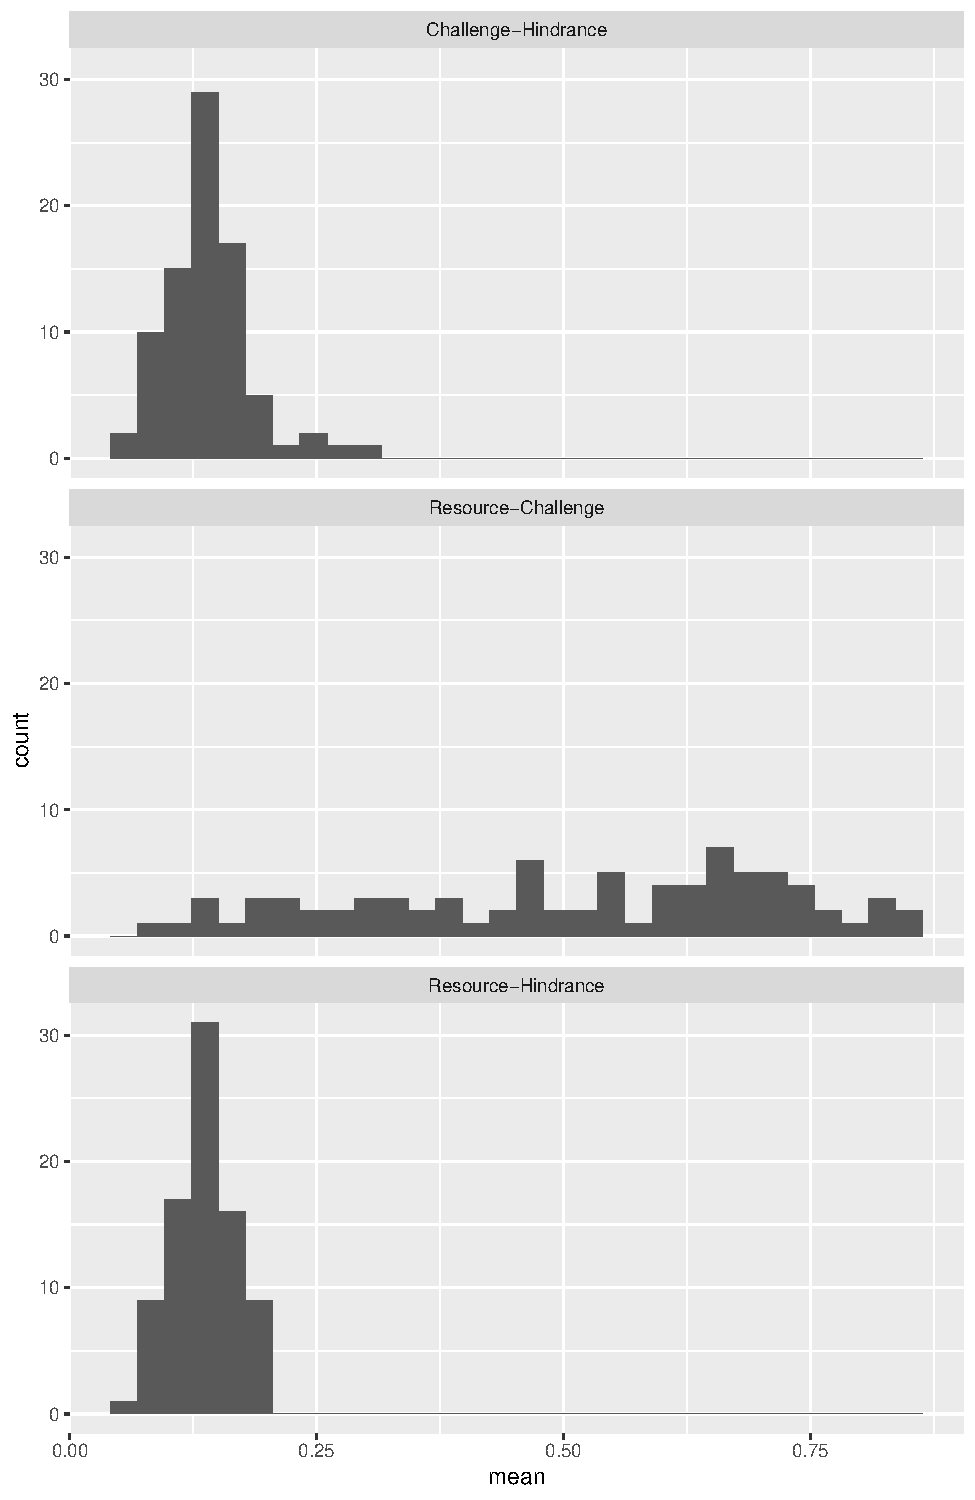
\includegraphics{convergence_files/figure-latex/percagree-1.pdf}
\caption{\label{fig:percagree}Percent convergence (characteristic rated consistently as, for example, both a resource and a hindrance.}
\end{figure}

Figure \ref{fig:percagree} shows that there was not much mutual agreement regarding characteristics viewed as both hindrances and resources (\(\bar{X}\) = 0.14) or as challenges and hindrances
(\(\bar{X}\) = 0.14). Alternatively, whether a characteristic was viewed as both a resource and a challenge exhibited greater consistency although also had quite a bit of variability (\(\bar{X}\) = 0.51, \emph{sd} = 0.21).

\begin{figure}
\centering
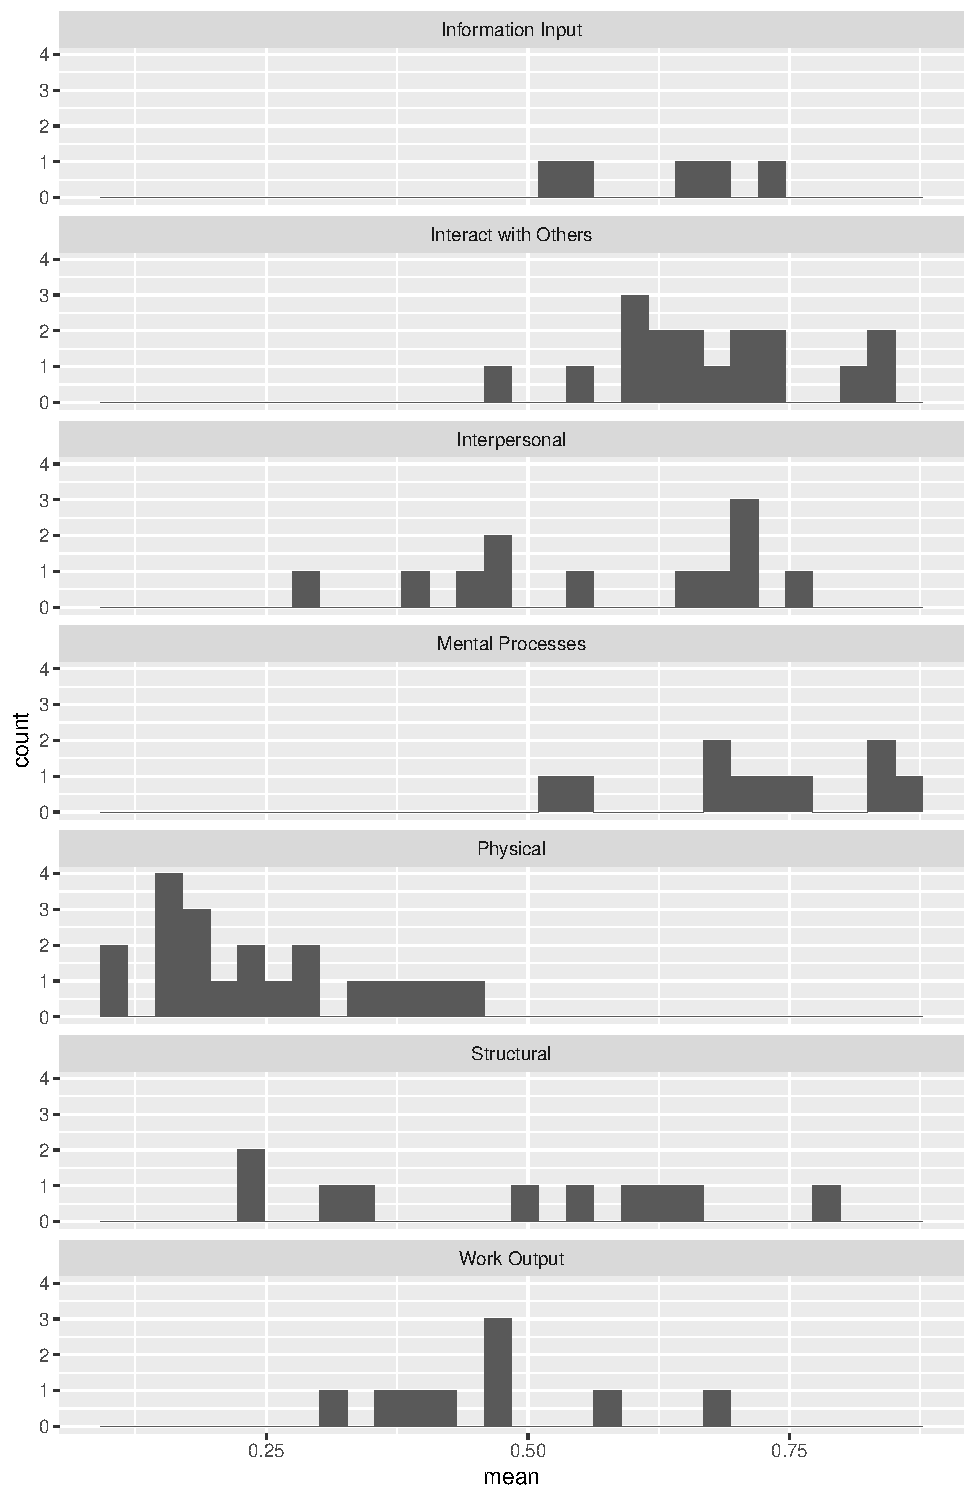
\includegraphics{convergence_files/figure-latex/recchall-1.pdf}
\caption{\label{fig:recchall}Resource and challenge agreement across ONet characteristic groupings (e.g., scales).}
\end{figure}

Figure \ref{fig:recchall} explores the possibility of moderation by \emph{type of characteristic rated} for the resource-challenge convergence. We categorized each characteristic by its ONet ``scale'' (one of seven), and the graph shows consistency across certain characteristics (for example, ) and non-convergence across other \emph{types} of characteristics (for example, ``Physical'' characteristics).

F ratio from a repeated measures ANOVA is \(F_(6, 3,402)\) = 613.5, \emph{p} \textless{} .001 (the subjects' effect was \(F_{(567, 3402)}\) = 6.13, \emph{p} \textless{} .001.

\hypertarget{discussion}{%
\section{Discussion}\label{discussion}}

The major goal of this paper was to further explore the relationships among total perceived challenge demands, hindrance demands, and resources and outcomes of engagement, stress, and burnout. Additionally, we considered whether resources and challenge demands were perceived as distinct, and finally, whether the patterns were similar across job categories/types of work. The results suggest a positive relationship between both resources and engagement (H1a), and challenge demands and engagement (H2a). Employers would benefit from understanding that at leas the perception of having ``more'' resources and more challenge demands in a job is highly associated with reported engagement. While not a causal relationship, it points to the potential value of these kinds of employee support nonetheless. The other relationships with outcomes of stress and burnout were not supported, suggesting that the sheer number of resources, challenges, and hindrances are not significantly related to these negative outcomes. It is possible that rather than volume, categorically some demands are more related to these outcomes than others.
Further, total resources were highly associated challenge demands (supporting H4). We could even argue, given the magnitude of the correlation, that they are capturing the same thing (74\% overlap with a correlation of .86). Need to also talk about our exploratory findings regarding patterns across job type

\hypertarget{limitations-and-future-directions}{%
\subsection{Limitations and Future Directions}\label{limitations-and-future-directions}}

As with any piece of research, the process and results have limitations, but also provide a variety of additional directions to pursue in the future. First, while a strength of this project, arguably, is the use of O\emph{Net items, practical considerations limited the number of job characteristics we could include in our survey. Future study could consider additional or other O}Net items. We conceptualized resources and demands in terms of perceived total amounts. It may be the case that certain kinds of resources or challenges are more strongly associated with engagement than others, and such, future research could explore the importance of resources/challenges categorically. Further, our study was limited to three outcomes of interest. It would be especially interesting to explore additional outcomes (e.g., job satisfaction) as well, or whether volume of resources and demands operationalized in this way are related to other behaviors (e.g., turnover intention, perceived organizational support, commitment).

\hypertarget{references}{%
\section*{References}\label{references}}
\addcontentsline{toc}{section}{References}

\hypertarget{refs}{}
\begin{CSLReferences}{1}{0}
\leavevmode\vadjust pre{\hypertarget{ref-abbas2019challenge}{}}%
Abbas, M., \& Raja, U. (2019). Challenge-hindrance stressors and job outcomes: The moderating role of conscientiousness. \emph{Journal of Business and Psychology}, \emph{34}(2), 189--201.

\leavevmode\vadjust pre{\hypertarget{ref-R-papaja}{}}%
Aust, F., \& Barth, M. (2022). \emph{Papaja: Prepare american psychological association journal articles with r markdown}. \url{https://github.com/crsh/papaja}

\leavevmode\vadjust pre{\hypertarget{ref-bakker2014job}{}}%
Bakker, A. B., \& Demerouti, E. (2014). Job demands--resources theory. \emph{Wellbeing: A Complete Reference Guide}, 1--28.

\leavevmode\vadjust pre{\hypertarget{ref-bakker2017job}{}}%
Bakker, A. B., \& Demerouti, E. (2017). Job demands--resources theory: Taking stock and looking forward. \emph{Journal of Occupational Health Psychology}, \emph{22}(3), 273.

\leavevmode\vadjust pre{\hypertarget{ref-bakker2007job}{}}%
Bakker, A. B., Hakanen, J. J., Demerouti, E., \& Xanthopoulou, D. (2007). Job resources boost work engagement, particularly when job demands are high. \emph{Journal of Educational Psychology}, \emph{99}(2), 274.

\leavevmode\vadjust pre{\hypertarget{ref-bakker2013weekly}{}}%
Bakker, A. B., \& Sanz-Vergel, A. I. (2013). Weekly work engagement and flourishing: The role of hindrance and challenge job demands. \emph{Journal of Vocational Behavior}, \emph{83}(3), 397--409.

\leavevmode\vadjust pre{\hypertarget{ref-bakker2003dual}{}}%
Bakker, A., Demerouti, E., \& Schaufeli, W. (2003). Dual processes at work in a call centre: An application of the job demands--resources model. \emph{European Journal of Work and Organizational Psychology}, \emph{12}(4), 393--417.

\leavevmode\vadjust pre{\hypertarget{ref-R-tinylabels}{}}%
Barth, M. (2022). \emph{Tinylabels: Lightweight variable labels}. \url{https://github.com/mariusbarth/tinylabels}

\leavevmode\vadjust pre{\hypertarget{ref-cavanaugh2000empirical}{}}%
Cavanaugh, M. A., Boswell, W. R., Roehling, M. V., \& Boudreau, J. W. (2000). An empirical examination of self-reported work stress among US managers. \emph{Journal of Applied Psychology}, \emph{85}(1), 65.

\leavevmode\vadjust pre{\hypertarget{ref-crawford2010linking}{}}%
Crawford, E. R., LePine, J. A., \& Rich, B. L. (2010). Linking job demands and resources to employee engagement and burnout: A theoretical extension and meta-analytic test. \emph{Journal of Applied Psychology}, \emph{95}(5), 834.

\leavevmode\vadjust pre{\hypertarget{ref-demerouti2001job}{}}%
Demerouti, E., Bakker, A. B., Nachreiner, F., \& Schaufeli, W. B. (2001). The job demands-resources model of burnout. \emph{Journal of Applied Psychology}, \emph{86}(3), 499.

\leavevmode\vadjust pre{\hypertarget{ref-gerich2017relevance}{}}%
Gerich, J. (2017). The relevance of challenge and hindrance appraisals of working conditions for employees' health. \emph{International Journal of Stress Management}, \emph{24}(3), 270.

\leavevmode\vadjust pre{\hypertarget{ref-kristensen2005copenhagen}{}}%
Kristensen, T. S., Borritz, M., Villadsen, E., \& Christensen, K. B. (2005). The copenhagen burnout inventory: A new tool for the assessment of burnout. \emph{Work \& Stress}, \emph{19}(3), 192--207.

\leavevmode\vadjust pre{\hypertarget{ref-lazarus1984stress}{}}%
Lazarus, R. S., \& Folkman, S. (1984). \emph{Stress, appraisal, and coping}. Springer publishing company.

\leavevmode\vadjust pre{\hypertarget{ref-pejtersen2010second}{}}%
Pejtersen, J. H., Kristensen, T. S., Borg, V., \& Bjorner, J. B. (2010). The second version of the copenhagen psychosocial questionnaire. \emph{Scandinavian Journal of Public Health}, \emph{38}(3\_suppl), 8--24.

\leavevmode\vadjust pre{\hypertarget{ref-podsakoff2007differential}{}}%
Podsakoff, N. P., LePine, J. A., \& LePine, M. A. (2007). Differential challenge stressor-hindrance stressor relationships with job attitudes, turnover intentions, turnover, and withdrawal behavior: A meta-analysis. \emph{Journal of Applied Psychology}, \emph{92}(2), 438.

\leavevmode\vadjust pre{\hypertarget{ref-R-base}{}}%
R Core Team. (2021). \emph{R: A language and environment for statistical computing}. R Foundation for Statistical Computing. \url{https://www.R-project.org/}

\leavevmode\vadjust pre{\hypertarget{ref-schaufeli2002measurement}{}}%
Schaufeli, W. B., Salanova, M., González-Romá, V., \& Bakker, A. B. (2002). The measurement of engagement and burnout: A two sample confirmatory factor analytic approach. \emph{Journal of Happiness Studies}, \emph{3}(1), 71--92.

\leavevmode\vadjust pre{\hypertarget{ref-searle2015merits}{}}%
Searle, B. J., \& Auton, J. C. (2015). The merits of measuring challenge and hindrance appraisals. \emph{Anxiety, Stress, \& Coping}, \emph{28}(2), 121--143.

\leavevmode\vadjust pre{\hypertarget{ref-selye1936syndrome}{}}%
Selye, H. (1936). A syndrome produced by diverse nocuous agents. \emph{Nature}, \emph{138}(3479), 32--32.

\leavevmode\vadjust pre{\hypertarget{ref-webster2011extending}{}}%
Webster, J. R., Beehr, T. A., \& Love, K. (2011). Extending the challenge-hindrance model of occupational stress: The role of appraisal. \emph{Journal of Vocational Behavior}, \emph{79}(2), 505--516.

\end{CSLReferences}


\end{document}
